\documentclass[10pt,a4paper]{article}

\usepackage{polski}
\usepackage[utf8]{inputenc}
\usepackage[polish]{babel}
\usepackage{hhline}
\usepackage{pgfplots}
\usepackage{multicol}
\usepackage{graphicx}
\usepackage{caption}
\usepackage{subcaption}
\usepackage{colortbl}
\usepackage{geometry}
\usepackage{listings}
\usepackage{mathtools}
\DeclarePairedDelimiter\ceil{\lceil}{\rceil}
\DeclarePairedDelimiter\floor{\lfloor}{\rfloor}
\geometry{a4paper, total={170mm,257mm}, left=20mm, top=20mm }


\author{Sebastian Maciejewski 132275 i Jan Techner 132332\\
grupa I1, zajęcia w środy o 9:45}
\title{Przetwarzanie rozproszone - projekt “Obsługa Pyrkonu”}
\date{15 maja 2019}
\setlength{\parindent}{0pt}
\newcommand{\forceindent}{\leavevmode{\parindent=3em\indent}}
\begin{document}
\maketitle
\section{Opis problemu}
Zadanie polega na implementacji systemu zarządzania biletami na Pyrkon i warsztaty, które się na nim odbywają. Procesy (uczestnicy) ubiegają się o jeden z b biletów na Pyrkon,
a następnie na kilka z rozróżnialnych warsztatów, z których każdy ma ograniczoną liczbę miejsc. Liczba warsztatów, miejsc na warsztatach i biletów na Pyrkon jest
w naszej implementacji losowana przez proces, który uruchamia wątek rozpoczęcia Pyrkonu.
Poniżej przedstawiony jest schemat działania i opis algorytmu.\\
\\
Działanie algorytmu rozpoczyna się od zgłoszenia przez każdy z procesów chęci rozpoczęcia nowego Pyrkonu.
W tym celu każdy proces wysyła wiadomość typu WANT\_TO\_BE\_HOST i czeka na p-1 (p jest ilością procesów)
pozytywnych odpowiedzi. Problemy z synchronizacją tego typu komunikacji rozwiązujemy dzięki algorytmowi
Ricarta-Agrawali i wykorzystaniu sekcji krytycznej (osobnej dla każdego procesu).
Wybrany w taki sposób proces zostaje hostem i wysyła informację HOST\_CHOSEN do reszty procesów,
po czym następuje inkrementacja numeru Pyrkonu - wysłanie do wszystkich informacji PYRKON\_START,
po której odebraniu pozostałe procesy inkrementują swoje numery Pyrkonu. Następnie host zwiększa 
swój numer Pyrkonu i tworzy wątek losujący.\\
\\
Ta procedura jest zobrazowana w górnej części poniższego diagramu, dodatkowy wątek (zaznaczony na niebiesko)
losuje ilość warsztatów, biletów na warsztaty i ilość biletów na Pyrkon, po czym przekazuje ją
wszystkim procesom za pomocą wiadomości PYRKON\_TICKETS i WORKSHOP\_TICKETS.\\
Każdy z procesów po odebraniu informacji o biletach wysyła wiadomość GOT\_TICKETS\_INFO i czeka
aż otrzyma taką wiadomość od reszty procesów. Dopiero wtedy mamy pewność, że wszyscy mają ten
sam numer Pyrkonu i te same (aktualne) informacje o biletach - można zatem rozpocząć procedurę 
ubiegania się o bilety.\\
\\
Każdy z Procesów informuje pozostałe o chęci wejścia na konwent (za pomocą wiadomości WANT\_PYRKON\_TICKET)
i po otrzymaniu odpowiedniej ilości ($p-b$) pozytywnych odpowiedzi zajmuje bilet. Następuje losowanie
ilości i numerów warsztatów, w których proces chce wziąć udział, po czym rozpoczyna się procedura ubiegania
się procesu o bilet na warsztaty. Jak widać na poniższym diagramie, kroki, które wykonuje proces są 
podobne do tych przy pobieraniu biletu na Pyrkon. Głównymi różnicami są tu typy wiadomości i fakt, że 
proces czeka na $p-w_i$ wiadomości ze zgodą na wejście na warsztat, gdzie $w_i$ to ilość biletów na $i$-ty warsztat.\\
Po otrzymaniu biletu i odczekaniu losowej ilości czasu (kiedy bierze udział w warsztacie), proces 
zwalnia bilet i, jeśli chce wziąć udział w jeszcze jakimś warsztacie, ponownie ubiega się o bilet,
tym razem na kolejny warsztat. Jeśli zaś proces przeszedł już wszystkie warsztaty, którymi był
zainteresowany, wówczas zwalnia bilet na Pyrkon (wysyła odpowiedź ze zgodą na wejście oczekującym procesom)
i wraca do momentu, w którym ubiegał się o zostanie hostem. Kiedy wszystkie procesy opuszczą Pyrkon,
cały opisany proces rozpoczyna się od nowa.


\newpage
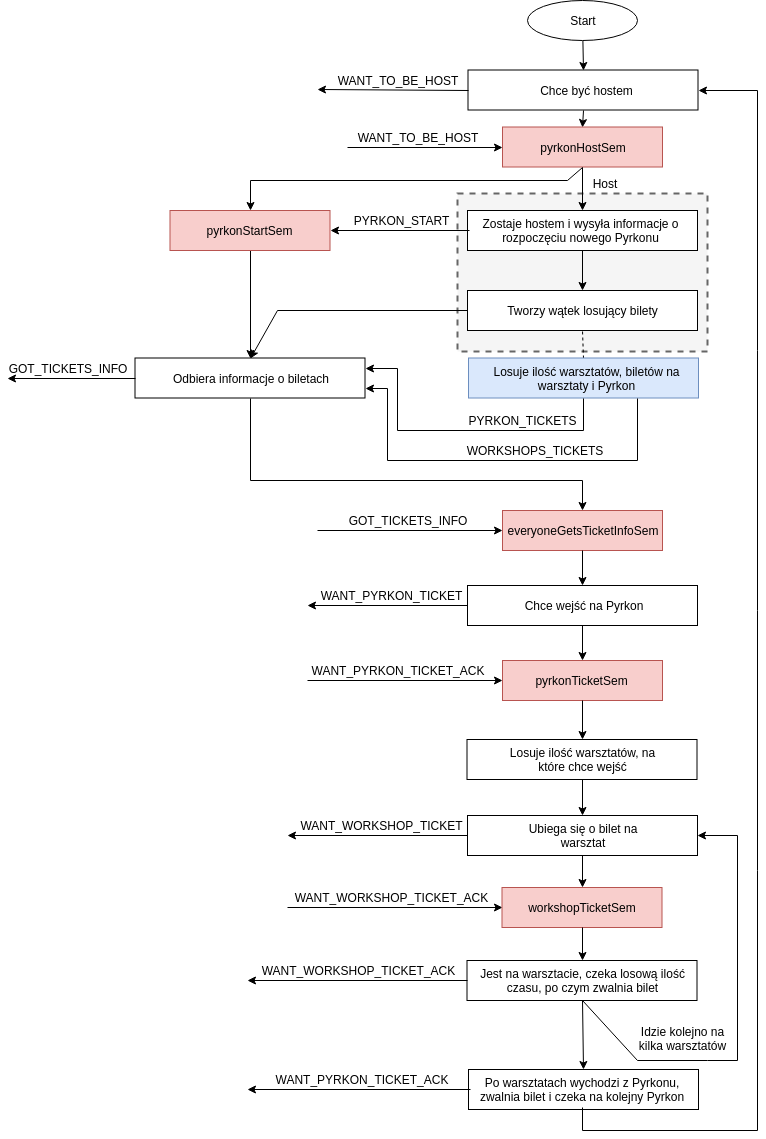
\includegraphics[height=\textheight]{diagram.png}


\end{document}